\section*{Image Restoration}

Image restoration attempts to restore images that have been degraded.

\begin{itemize}
  \item Identify the degradation process and \textbf{attempt to reverse it}
  \item Similar to image enhancement, but \textbf{more objective}
\end{itemize}

\subsection*{Noise and Images}

The sources of noise in digital images arise during image acquisition
(digitization) and transmission
\begin{itemize}
  \item Imaging sensors can be affected by ambient conditions
  \item Interference can be added to an image during transmission
\end{itemize}

\subsection*{Noise in Images}

We can consider a noisy image to be modeled as follows:

\begin{equation*}
  g(x, y) = f(x, y) + \eta(x, y)
\end{equation*}

(i) $f(x, y) \rightarrow$ original image pixel (ii) $\eta(x, y)
\rightarrow$ the noise term and (iii) $g(x, y) \rightarrow$ resulting
noisy pixel

If we can \textbf{estimate the model} that the noise in an image is
based on, it will help us to figure out \textbf{how to restore the image}.

\subsection*{Mean Filters for Restoration}

\begin{itemize}
  \item \textbf{Arithmetic Mean Filter:} Smooths local variations;
    blurs the image to reduce noise.
    \begin{equation*}
      \hat{f}(x, y) = \frac{1}{mn} \sum_{(s, t) \in S_{xy}} g(s, t)
    \end{equation*}

  \item \textbf{Geometric Mean Filter:} Comparable to the arithmetic
    mean filter, tends to lose less image detail.
    \begin{equation*}
      \hat{f}(x, y) = \left( \prod_{(s, t) \in S_{xy}} g(s, t) \right)^{1/(mn)}
    \end{equation*}

  \item \textbf{Harmonic Mean Filter:} Works well for \textbf{salt
    noise}, but \textbf{fails} for \textbf{pepper noise}. Also does
    well for other kinds of noise, such as \textbf{Gaussian noise}.
    \begin{equation*}
      \hat{f}(x, y) = \frac{mn}{\sum_{(s, t) \in S_{xy}} 1/g(s, t)}
    \end{equation*}

  \item \textbf{Contraharmonic Mean Filter:} Takes a parameter $Q$,
    the \textbf{order} of the filter.
    \begin{itemize}
      \item $Q > 0 \rightarrow$ removes \textbf{pepper noise}
      \item $Q < 0 \rightarrow$ removes \textbf{salt noise}
      \item Wrong value of $Q$ can have drastic results
    \end{itemize}

    \begin{equation*}
      \hat{f}(x, y) = \frac{\sum_{(s, t) \in S_{xy}} g(s, t)^{Q +
      1}}{\sum_{(s, t) \in S_{xy}} g(s, t)^Q}
    \end{equation*}
\end{itemize}

\subsubsection*{Drawbacks with Mean Filtering}

\begin{itemize}
  \item A single pixel with a very \textbf{unrepresentative value}
    can \textbf{significantly affect} the mean value of all the
    pixels in its neighborhood
  \item When the filter neighborhood \textbf{straddles an edge}, the
    filter will \textbf{interpolate new values} for pixels on the
    edge and so will blur that edge; may be a problem if sharp edges
    are required in the output
\end{itemize}

\subsection*{Degradation Models}

Given: (i) corrupted image $g(x, y)$ (ii) some knowledge about the
degradataion function $H$ (iii) some knowledge about the noise $\eta(x, y)$

Objective: obtain an $f(x, y)$ estimate of the original image

\begin{itemize}
  \item \textbf{Spatial domain:} $g(x, y) = h(x, y) * f(x, y) + \eta(x, y)$
  \item \textbf{Frequency domain:} $G(u, v) = H(u, v) * F(u, v) + N(u, v)$
\end{itemize}

Spatial filtering is the method of noise when only additive noise if
present. Enhancement \& restoration become \textbf{almost
indistinguishable disciplines} in this particular case.

\subsection*{Noise Models}

\begin{itemize}
  \item Images are often degraded by \textbf{random noise} with
    \textbf{probabilistic characteristics}
  \item Noise can occur during (i) image capture, (ii) transmission
    or (ii) processing
  \item May be (i) dependent on or (ii) independent of image content
\end{itemize}

\subsubsection*{White Noise}

\begin{itemize}
  \item Simplest noise
  \item Constant power spectrum (its intensity \textbf{does not
    decrease} with \textbf{increasing frequency})
  \item Frequently applied as a \textbf{crude approximation} of image
    noise in most cases
  \item Advantage: simplifies the calculations
\end{itemize}

\subsubsection*{Gaussian Noise}

\begin{equation*}
  p(z) =\frac{1}{\sigma\sqrt{2 \pi}} e^{-(z - \mu)^2/2 \sigma^2}
\end{equation*}

(i) $z \rightarrow$ gray level (ii) $\mu \rightarrow$ mean of average
value of $z$ (iii) $\sigma \rightarrow$ standard deviation of $z$
(iv) 70\% of its values: $[ \mu \pm \sigma ]$ (v) 95\% of its values:
$[ \mu \pm 2\sigma ]$

\begin{itemize}
  \item Very good approximation of noise that occurs in most cases
  \item Probability of the random variable is given by the Gaussian function
\end{itemize}

\subsubsection*{Rayleigh Noise}

\begin{equation*}
  p(z) =
  \begin{cases}
    \frac{2}{b} (z-a) e^{-(z-a)^2/b} & \text{if } z \geq a \\
    0 & \text{otherwise}
  \end{cases}
\end{equation*}

(i) $\mu = a + \sqrt{\pi b / 4}$ (ii) $\sigma^2 = \frac{b(4 - \pi)}{4}$

\subsubsection*{Gamma Noise}

\begin{equation*}
  p(z) =
  \begin{cases}
    \frac{a^b z^{b-1}}{(b-1)!} e^{-az} & \text{if } z \geq a \\
    0 & \text{otherwise}
  \end{cases}
\end{equation*}

(i) $\mu = \frac{b}{a}$ (ii) $\sigma^2 = \frac{b}{a^2}$

\subsubsection*{Exponential Noise}

\begin{equation*}
  p(z) =
  \begin{cases}
    ae^{-az} & \text{if } z \geq 0 \\
    0 & \text{otherwise}
  \end{cases}
\end{equation*}

(i) $\mu = \frac{1}{a}$ (ii) $\sigma^2 = \frac{1}{a^2}$

\subsubsection*{Uniform Noise}

\begin{equation*}
  p(z) =
  \begin{cases}
    \frac{1}{b-a} & \text{if } a \leq z \leq b \\
    0 & \text{otherwise}
  \end{cases}
\end{equation*}

(i) $\mu = \frac{a + b}{2}$ (ii) $\sigma^2 = \frac{(b - a)^2}{12}$

\subsubsection*{Impulse Noise}

Randomly scattered \textbf{white} (\enquote{salt}) or \textbf{black}
(\enquote{pepper}) pixels over the image.

\begin{equation*}
  p(z) =
  \begin{cases}
    P_a & \text{if } z = a \\
    P_b & \text{if } z = b \\
    P_c & \text{otherwise}
  \end{cases}
\end{equation*}

\begin{itemize}
  \item \textbf{Bipolar:} $P_a \neq 0, P_b \neq 0$
  \item \textbf{Unipolar (salt and pepper):} $P_a = 0$ or $P_b = 0$
\end{itemize}

\subsection*{Estimation of Noise Parameters}

\begin{enumerate}
  \item The shape of the histogram identifies the closest PDF match
  \item Get mean \& variance of the gray levels
  \item Use $\mu$ \& $\sigma^2$ to solve for the parameters a \& b
\end{enumerate}

\textbf{Gaussian noise}: mean \& variance only

\textbf{Impulse noise}: the actual probability of occurrence of white
\& black pixels are needed

\subsection*{Order Statistics Filters for Restoration}

The response is based on the \textbf{ordering} of the pixel values in
the image area encompassed by the filter mask.

\begin{itemize}
  \item \textbf{Median Filter:} Removes salt and pepper noise
    \begin{equation*}
      \hat{f}(x, y) = \text{median}_{(a, b) \in S} \left\{ g(x - a, y
      - b) \right\}
    \end{equation*}

  \item \textbf{Max Filter:} Removes pepper noise
    \begin{equation*}
      \hat{f}(x, y) = \max_{(a, b) \in S} \left\{ g(x - a, y - b) \right\}
    \end{equation*}

  \item \textbf{Min Filter:} Removes salt noise
    \begin{equation*}
      \hat{f}(x, y) = \min_{(a, b) \in S} \left\{ g(x - a, y - b) \right\}
    \end{equation*}

  \item \textbf{Midpoint Filter:} Order statistics + averaging; works
    best for Gaussian or uniform noise
    \vspace{-0.1em}
    \begin{equation*}
      \frac{1}{2} \bigg[ \max_{(a, b) \in S} \left\{
        g(x - a, y - b) \right\} + \min_{(a, b) \in S} \left\{ g(x - a,
      y - b) \right\} \bigg]
    \end{equation*}

  \item \textbf{Alpha-trimmed Mean Filter:} Delete the $d/2$ lowest
    and $d/2$ highest gray level values of $g(x - a, y - b)$. Useful
    for situations involving multiple types of noise.

    \begin{equation*}
      \hat{f}(x, y) = \frac{g_r(x, y)}{mn - d}
    \end{equation*}

    $g_r \rightarrow$ sum of the remaining pixel values
\end{itemize}

\subsubsection*{Drawbacks with Order Statistics Filters}

\begin{itemize}
  \item Relatively expensive and complex to compute.
  \item To find the median it is necessary to \textbf{sort all the
    values} in the neighborhood into numerical order
  \item Sorting is relatively slow, even with fast sorting algorithms
    such as \textbf{quicksort}
  \item \textbf{Possible remedy:} When the filter is slid across the
    image, many of the pixels in the window are the same from one
    step to the next; the relative ordering of these with each other
    do not change
\end{itemize}

\subsection*{Adaptive Filtering}

Changing the behavior according to gray level values under the filter mask.

\begin{equation*}
  m_f + \frac{\sigma_f^2}{\sigma_f^2 + \sigma_g^2} (g - m_f)
\end{equation*}

\begin{itemize}
  \item $m_f \rightarrow$ mean under the mask
  \item $\sigma_f^2 \rightarrow$ variance under the mask
    (\enquote{local variance})
  \item $g \rightarrow$ current (grayscale) pixel value
  \item $\sigma_g^2 \rightarrow$ variance of the image
\end{itemize}

Insights:

\begin{itemize}
  \item $\sigma_f^2$ high $\rightarrow$ fraction is close to $1$,
    output is closer to \textbf{original value} ($g$), significant
    details (e.g. edges).

  \item $\sigma_f^2$ low $\rightarrow$ fraction is close to $0$,
    output is closer to \textbf{mean value} ($m_f$), smooths out noise.

  \item $\sigma_g^2$ often unknown; taken as the \textbf{mean} of all
    values of $\sigma_f^2$ in the image.
\end{itemize}

\subsubsection*{Variant}

Pratically, a \textbf{variant} of adaptive filtering is used:

\begin{equation*}
  m_f + \frac{\max \{0, \sigma_f^2 - \sigma_g^2 \}}{\max\{\sigma_f^2
  + \sigma_g^2\}} (g - m_f)
\end{equation*}

Purposes:

\begin{itemize}
  \item Removes salt and pepper noise
  \item Smooths other noise that may not be impulsive
  \item Reduces distortion (e.g. excessive thickening/thinning of boundaries)
\end{itemize}

\subsubsection*{Adaptive Median Filter}

\begin{itemize}
  \item The median filter performs relatively well on \textbf{impulse noise}
    as long as the \textbf{spatial density} of the impulse noise is
    \textbf{not large}
  \item The \textbf{adaptive median filter} can handle much more spatially
    dense impulse noise
  \item It also performs some \textbf{smoothing} for non-impulse noise
  \item Key insight: \textbf{filter size changes} depending on the
    characteristics of the image
\end{itemize}

\textbf{Level A}

\begin{enumerate}
  \item $A_1 = z_\text{med} - z_{min}$
  \item $A_2 = z_\text{med} - z_{max}$
  \item If $A_1 > 0$ and $A_2 < 0$, go to level B
  \item Else increase the window size
  \item If window size $\leq S_\text{max}$, repeat level A
  \item Else output $z_\text{med}$
\end{enumerate}

\textbf{Level B}

\begin{enumerate}
  \item $B_1 = z_\text{xy} - z_\text{min}$
  \item $B_2 = z_\text{xy} - z_\text{max}$
  \item If $B_1 > 0$ and $B_2 < 0$, output $z_\text{xy}$
  \item Else output $z_\text{med}$
\end{enumerate}

\subsection*{Periodic Noise}

\begin{itemize}
  \item Typically arises due to \textbf{electrical or electromagnetic
    interference}
  \item Effect: regular noise patterns in an image
  \item \textbf{Frequency domain techniques} most effective
\end{itemize}

\subsection*{Band-Reject Filters}

Removes a particular range of frequencies from the image

\textbf{Ideal band-reject filter:}

\begin{equation*}
  H(u,v)=
  \begin{cases}
    1 & \text{if } D(u,v) < D_0 - \dfrac{W}{2}\\
    0 & \text{if } D_0 - \dfrac{W}{2} \le D(u,v) \le D_0 + \dfrac{W}{2}\\
    1 & \text{if } D(u,v) > D_0 + \dfrac{W}{2}
  \end{cases}
\end{equation*}

\begin{figure}[H]
  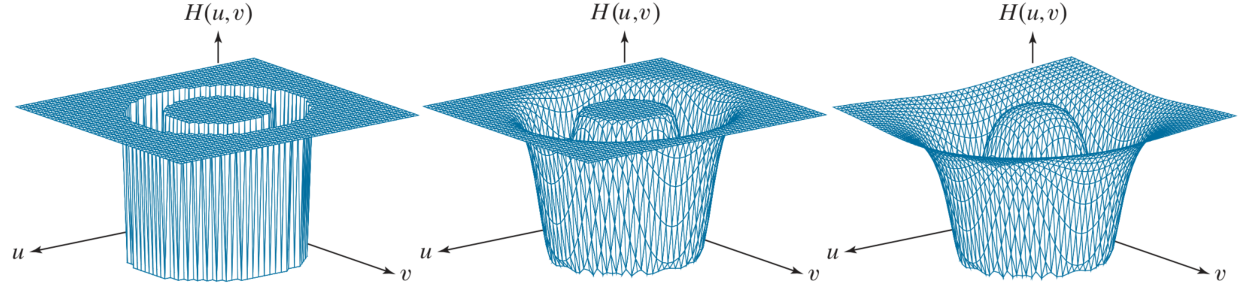
\includegraphics[width=\linewidth]{images/band_reject_filters.png}
  \caption{Ideal, Gaussian and Butterworth band-reject filters}
\end{figure}

\subsection*{Degradation}

$G(u, v) = F(u, v) * H(u, v)$

(i) $G(u, v) \rightarrow$ degraded image (ii) $F(u, v) \rightarrow$
original image (iii) $H(u, v) \rightarrow$ filter (degradation function)

Goal: $G$ and $H$ are known, obtain $F$

\subsubsection*{Inverse Filtering}

Simplest approach to restoration.

\begin{equation*}
  \hat{F}(u, v) = \frac{G(u, v)}{H(u, v)} = F(u, v) + \frac{N(u, v)}{H(u, v)}
\end{equation*}

$N(u, v) \rightarrow$ random function whose Fourier transform is
unknown; we cannotrecover the undegraded image even if $H(u, v)$ is known.

\begin{itemize}
  \item \textbf{Problem:} If $H(u, v)$ approaches 0, $\frac{N(u, v)}{H(u,
    v)}$ dominates the estimate $\hat{F}(u, v)$.
  \item \textbf{Solution:} Limit the analysis to frequencies near the origin.
\end{itemize}

\textbf{Approaches:}

\begin{itemize}
  \item \textbf{Low-pass filtering:} Uses filter $L(u, v)$
    \begin{equation*}
      F(u, v) = \frac{G(u, v)}{H(u, v)}L(u, v)
    \end{equation*}
  \item \textbf{Thresholding:} Using only filter frequencies near the origin
    \begin{equation*}
      F(u, v) =
      \begin{cases}
        \frac{G(u, v)}{H(u, v)} & \text{if } D(u, v) < d \\
        G(u, v) & \text{otherwise}
      \end{cases}
    \end{equation*}
\end{itemize}

\textbf{Weaknesses:}

\begin{itemize}
  \item Inverse filtering is \textbf{not robust} to noise (doesn't
    explicitly handle it)
  \item Easily corrupted by random noise
    \begin{gather*}
      G(u, v) = F(u, v) * H(u, v) + N(u, v) \\
      F(u, v) = \frac{G(u, v) - N(u, v)}{H(u, v)}
    \end{gather*}
  \item The noise can completely dominate the output
\end{itemize}

\subsubsection*{Wiener Filtering}

Aims to minimize the \textbf{mean square error} between the original
image and the restored image.

\begin{equation*}
  \hat{F}(u, v) = \bigg[ \frac{1}{H(u, v)} \frac{|H(u, v)|^2}{|H(u, v)|^2 + K} \bigg] G(u, v)
\end{equation*}

$K \rightarrow$ specified constant
